Ultra-Low Leakage (ULL) logic aims to reduce the leakage current down to physical limit.

\begin{columns}
	\begin{column}{0.5\textwidth}
		\begin{figure}
			\centering
			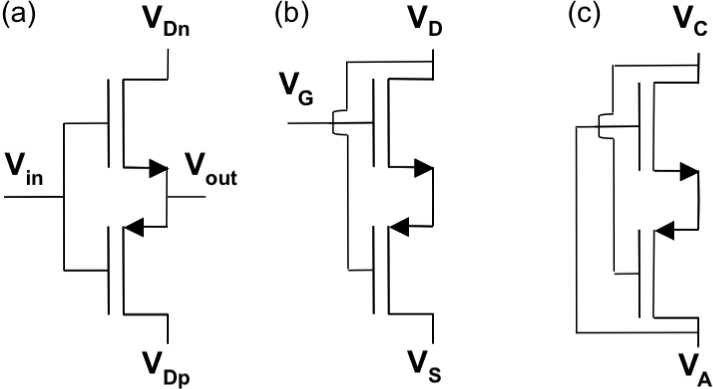
\includegraphics[width=\columnwidth]{../../images/ULLdevices.png}
			\caption{A selection of devices exploiting ultra-low leakage. (a) Voltage Follower, (b) Transistor, (c) Diode \cite{DisruptiveULL}}
			\label{fig:ulldevices}
		\end{figure}
	\end{column}
	\begin{column}{0.5\textwidth}
	\end{column}
\end{columns}

\begin{columns}
	\begin{column}{0.5\textwidth}
	\end{column}
	\begin{column}{0.5\textwidth}
\begin{figure}
	\centering
	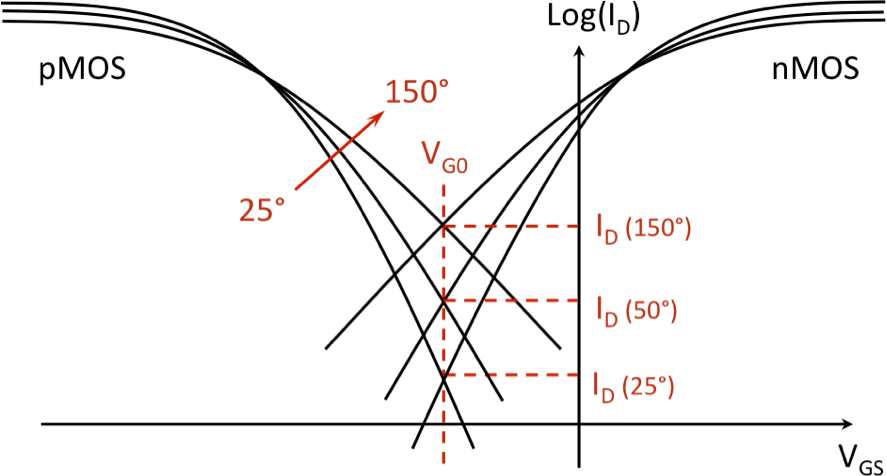
\includegraphics[width=\columnwidth]{../../images/intersectiongraph.png}
	\caption{A graph showing the autobiasing of $V_{gs}$ as temperature changes \cite{DisruptiveULL}}
	\label{fig:ullintersect}
\end{figure}
	\end{column}
\end{columns}
